% KJM: I moved this here to get the placement right
\begin{figure*}[h]
  \centering
  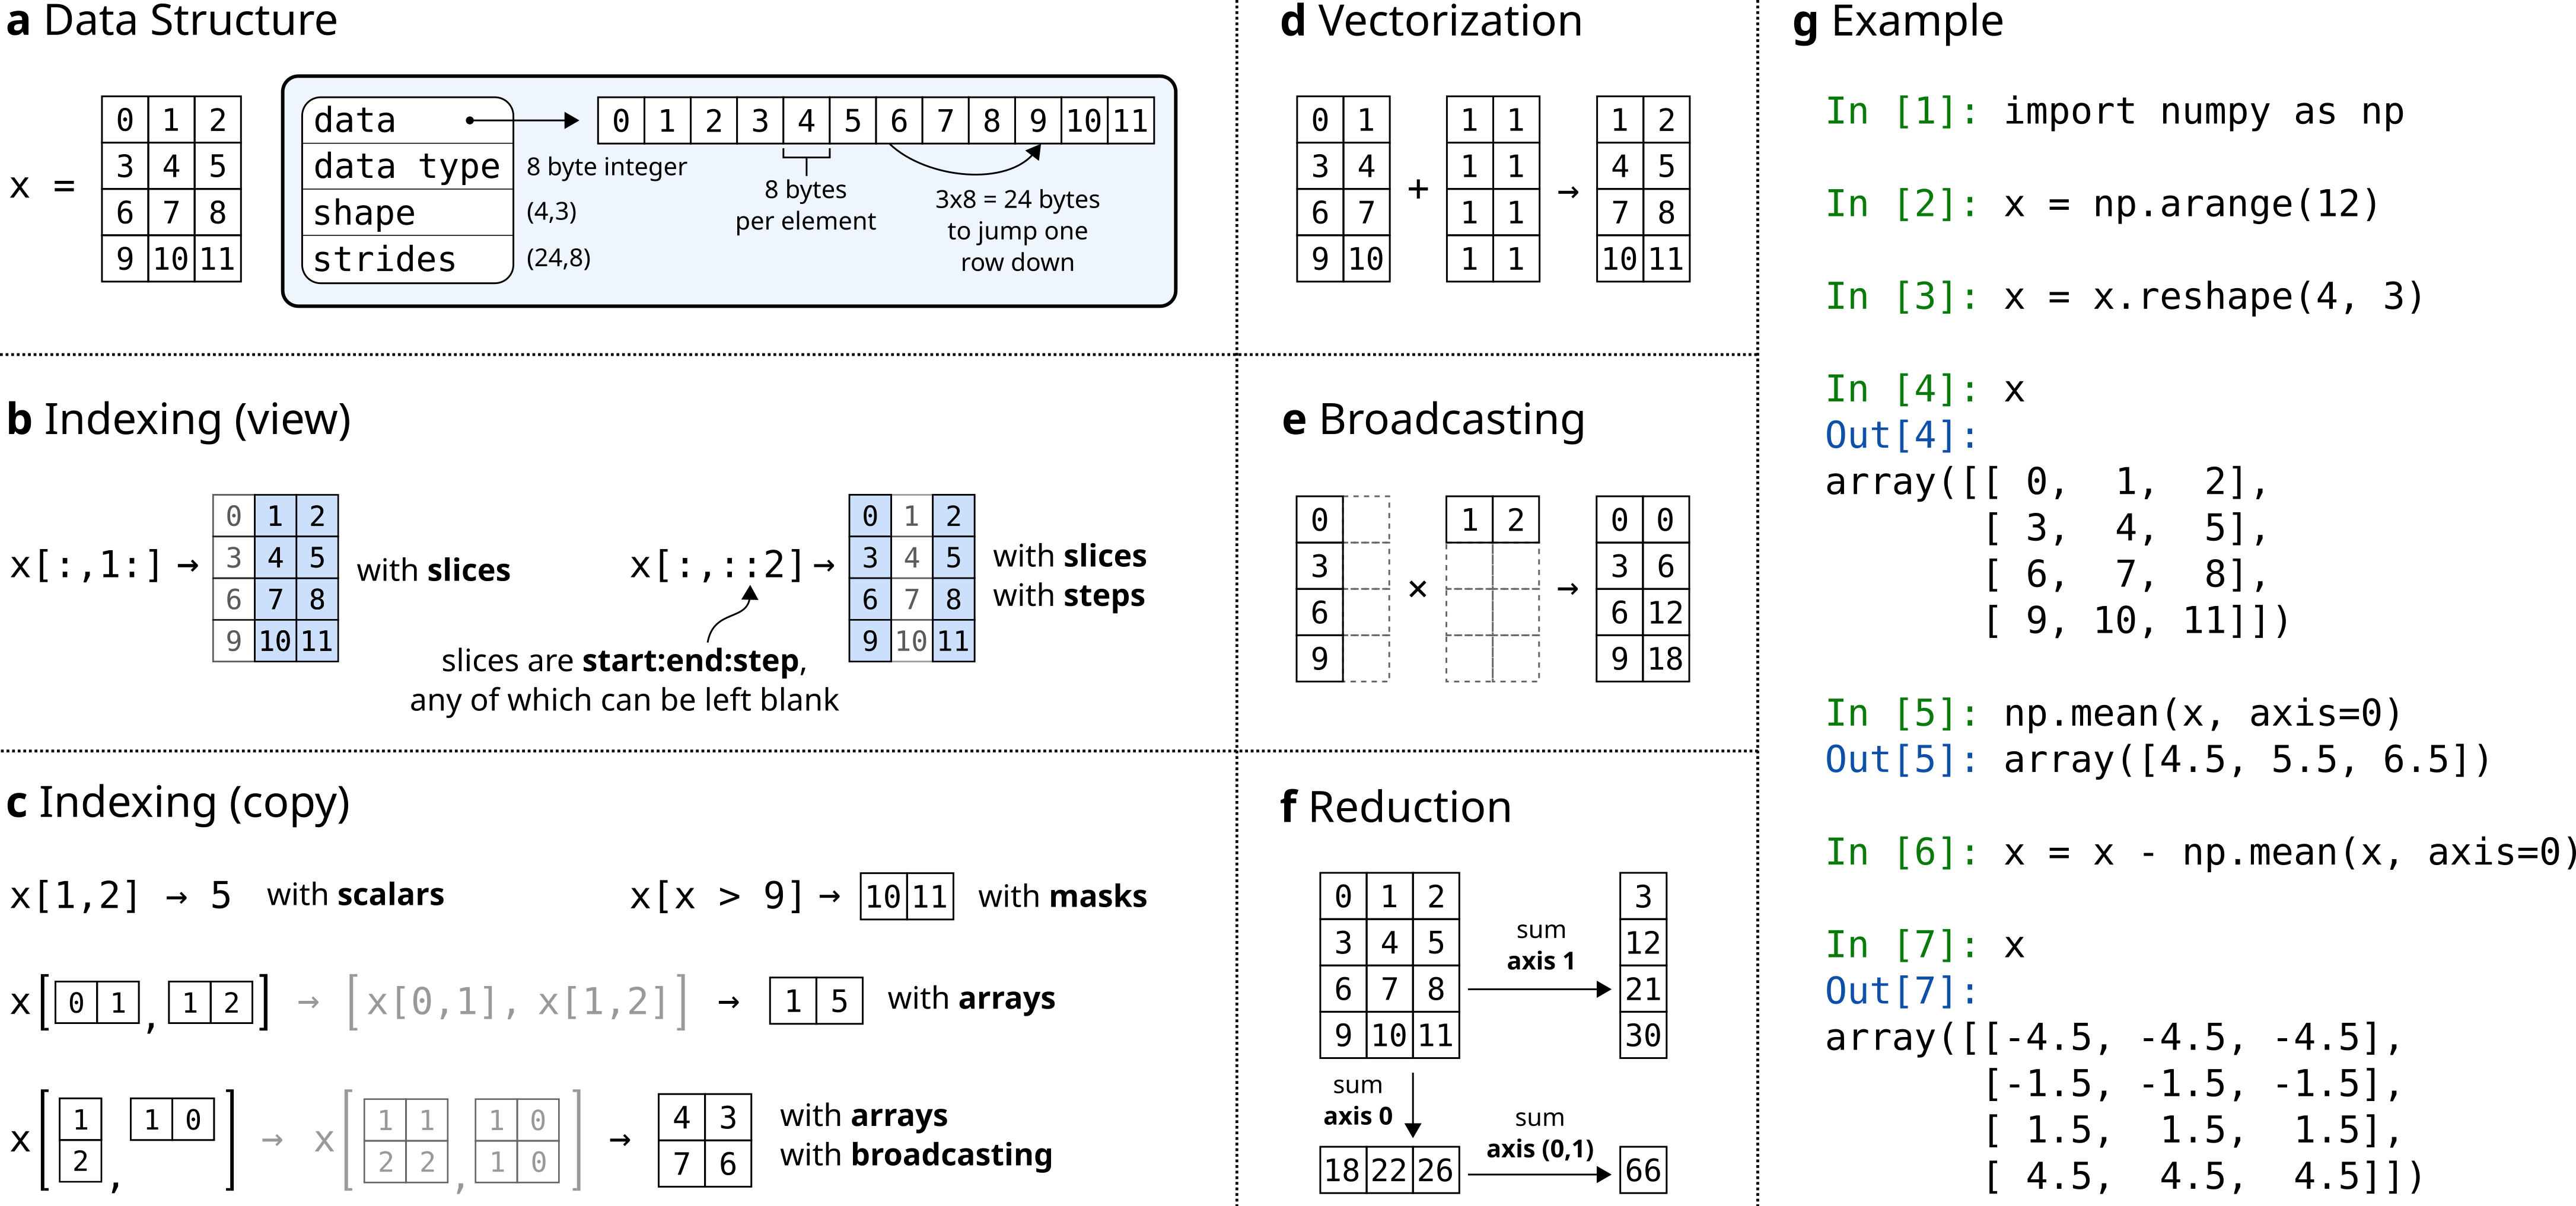
\includegraphics[width=\textwidth]{static/sketches/concepts}
  \caption{\textbf{The NumPy array incorporates several fundamental array concepts.}
    \textbf{a,} The NumPy array data structure and its associated metadata fields.
    \textbf{b,} Indexing an array with slices and steps. These
  operations return a \emph{view} of the original data.
    \textbf{c,} Indexing an array with masks, scalar coordinates, or
  other arrays, so that it returns a copy of the original data. In the
  bottom example, an array is indexed with other arrays; this broadcasts the indexing arguments before performing the lookup.
    \textbf{d,} Vectorization efficiently applies operations to groups
  of elements.
    \textbf{e,} Broadcasting in the multiplication of two-dimensional arrays.
    \textbf{f,} Reduction operations act along one or more axes. In this
    example, an array is summed along select axes to produce a vector, or along two axes consecutively to
    produce a scalar.
    \textbf{g,} Example NumPy code, illustrating some of these concepts.
   }
  \label{fig:array-concepts}
\end{figure*}

Two Python array packages existed before NumPy.
The Numeric package began in the mid-1990s and provided an array object and array-aware functions
in Python, written in C, and linking to standard fast implementations of linear
algebra \cite{dubois1996numerical,Numericmanual}.
One of its earliest uses was to steer C++ applications for
inertial confinement fusion research at
Lawrence Livermore National Laboratory \cite{yang1997steering}.
To handle large astronomical images coming from the Hubble Space Telescope,
a reimplementation of Numeric, called Numarray, added
support for structured arrays, flexible indexing, memory mapping, byte-order variants,
more efficient memory use, flexible IEEE error handling capabilities, and
better type casting rules \cite{greenfield2003numarray}.
While Numarray was highly compatible with Numeric, the two packages had enough
differences that it divided the community, until 2005, when NumPy emerged as a
``best of both worlds'' unification \cite{oliphant2006guide}---combining
Numarray's features with Numeric's performance on small arrays and its rich C
\emph{Application Programming Interface} (API).

Now, fifteen years later, NumPy underpins almost every Python library that does scientific or
numerical computation including SciPy \cite{virtanen2020scipy},
Matplotlib \cite{hunter2007matplotlib}, pandas \cite{mckinney-proc-scipy-2010},
scikit-learn \cite{pedregosa2011scikit}, and
scikit-image \cite{vanderwalt2014scikit}.
It is a community-developed, open-source library, which provides a
multidimensional Python array object along with array-aware functions
that operate on it.
Because of its inherent simplicity, the NumPy array is
the \emph{de facto} exchange format for array data in Python.

NumPy operates on in-memory arrays using the CPU. To utilize modern,
specialized storage and hardware, there has been a recent
proliferation of Python array packages. Unlike with the Numarray and
Numeric divide, it is now much harder for these new libraries to
fracture the user community---given how much work already builds
on top of NumPy.  However, to provide the ecosystem with access to
new and exploratory technologies, NumPy is transitioning into a
central coordinating mechanism that specifies a well-defined array
programming API and
dispatches it, as appropriate, to specialized array implementations.

\section*{NumPy arrays}

The NumPy array is a data structure that efficiently stores and accesses
multidimensional arrays \cite{vanderwalt2011numpy}, also known as tensors, and
enables a wide variety of scientific computation.
It consists of a pointer to memory, along with metadata used to interpret the
data stored there, notably {\em data type}, {\em shape}, and {\em strides}
(Fig.~\ref{fig:array-concepts}a).

The \emph{data type} describes the nature of elements stored in an array.
An array has a single data type, and each array element occupies the same
number of bytes in memory.
Examples of data types include real and complex numbers (of lower and higher
precision), strings, timestamps, and pointers to Python objects.

The \emph{shape} of an array determines the number of elements along each axis,
and the number of axes is the array's dimensionality.
For example, a vector of numbers can be stored as a one-dimensional array of
shape $N$, while color videos are four-dimensional arrays of shape
$(T, M, N, 3)$.

\emph{Strides} are necessary to interpret computer memory, which stores elements
linearly, as multidimensional arrays.
It describes the number of bytes to move forward in memory to jump from row to
row, column to column, and so forth.
Consider, for example, a 2-D array of floating-point numbers with shape
$(4, 3)$, where each element occupies 8 bytes in memory.
To move between consecutive columns, we need to jump forward 8 bytes in memory,
and to access the next row $3 \times 8 = 24$ bytes.
The strides of that array are therefore $(24, 8)$.  NumPy can
store arrays in either C or Fortran memory order, iterating
first over either rows or columns.  This allows external libraries
written in those languages to access NumPy array data in memory directly.

Users interact with NumPy arrays using {\em indexing} (to access
subarrays or individual elements), {\em operators} (e.g., $+$, $-$, $\times$
for vectorized operations and $@$ for matrix multiplication), as well as {\em array-aware functions};
together, these provide an easily readable, expressive, high-level API for
array programming, while NumPy
deals with the underlying mechanics of making operations fast.

\emph{Indexing} an array returns single elements, subarrays, or elements that satisfy
a specific condition (Fig.~\ref{fig:array-concepts}b).
Arrays can even be indexed using other arrays (Fig.~\ref{fig:array-concepts}c).
Wherever possible, indexing that retrieves a subarray returns a {\em view} on
the original array, such that data is shared between the two arrays.
This provides a powerful way to operate on subsets of array data while
limiting memory usage.

To complement the array syntax, NumPy includes functions that perform
\emph{vectorized} calculations on arrays, including arithmetic, statistics, and
trigonometry (Fig.~\ref{fig:array-concepts}d).
Vectorization---operating on whole arrays rather than their individual
elements---is essential to array programming.
This means that operations that would take many tens of lines to express in
languages such as C can often be implemented as a single, clear Python
expression.
This results in concise code and frees users to focus on the details of
their analysis, while NumPy handles looping over array elements near-optimally,
taking into consideration, for example, strides, to best utilize the
computer's fast cache memory.

When performing a vectorized operation (such as addition) on two arrays with
the same shape, it is clear what should happen.
Through \emph{broadcasting}, NumPy allows the dimensions to differ, while
still producing results that appeal to intuition.
A trivial example is the addition of a scalar value to an array, but broadcasting also
generalizes to more complex examples such as scaling each column of an array
or generating a grid of coordinates.
In broadcasting, one or both arrays are virtually duplicated (that is, without
copying any data in memory), so that the shapes of the operands match
(Fig.~\ref{fig:array-concepts}d).
Broadcasting is also applied when an array is indexed using arrays of
indices (Fig.~\ref{fig:array-concepts}c).

Other array-aware functions, such as \texttt{sum}, \texttt{mean}, and \texttt{maximum}, perform
element-by-element \emph{reductions}, aggregating results across one,
multiple, or all axes of a single array.
For example, summing an $n$-dimensional array over $d$ axes results in a
$(n-d)$-dimensional array (Fig.~\ref{fig:array-concepts}f).

NumPy also includes array-aware functions for creating, reshaping, concatenating, and padding
arrays; searching, sorting, and counting data; and reading and writing files.
It provides extensive support for generating pseudorandom numbers,
includes an assortment of probability distributions, and
performs accelerated linear algebra, utilizing one of several backends
such as OpenBLAS \cite{wang2013augem,xianyi2012model} or Intel MKL optimized
for the CPUs at hand.

Altogether, the combination of a simple in-memory array
representation, a syntax that closely mimics mathematics, and a
variety of array-aware utility functions forms a productive and
powerfully expressive array programming language.

\begin{figure}
  \centering
  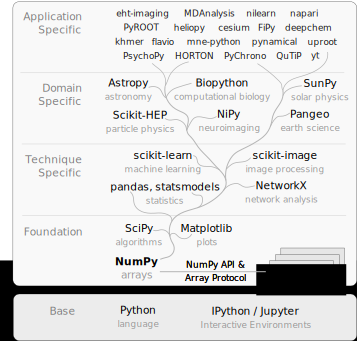
\includegraphics[width=.5\textwidth]{static/sketches/ecosystem}
  \caption{\textbf{NumPy is the base of the scientific Python ecosystem.}
   Essential libraries and projects that depend on NumPy's API gain access to new array
   implementations that support NumPy's array protocols (Fig.~\ref{fig:array-protocol}).
  }
  \label{fig:ecosystem}
\end{figure}

\section*{Scientific Python ecosystem}

Python is an open-source, general-purpose, interpreted programming language
well-suited to standard programming tasks such as cleaning data,
interacting with web resources, and parsing text.
Adding fast array operations and linear algebra allows scientists to do all
their work within a single language---and one that has the advantage of
being famously easy to learn and teach, as witnessed by its adoption
as a primary learning language in many universities.

Even though NumPy is not part of Python's standard library,
it benefits from a good relationship with the Python developers.
Over the years, the Python language has added new features and
special syntax so that NumPy would have a more succinct and 
easier to read array notation.
Since it is not part of the standard library, NumPy is able to
dictate its own release policies and development patterns.

SciPy and Matplotlib are tightly coupled with NumPy---in terms of
history, development, and use.
SciPy provides fundamental algorithms for scientific computing,
including mathematical, scientific, and engineering routines.
Matplotlib generates publication-ready figures and visualizations.
The combination of NumPy, SciPy, and Matplotlib, together with
an advanced interactive environment like IPython \cite{perez2007ipython},
or Jupyter \cite{Kluyver:2016aa}, provides a solid foundation for array
programming in Python.
The scientific Python ecosystem (Fig.~\ref{fig:ecosystem}) builds on top of
this foundation to provide several, widely used \emph{technique specific}
libraries\cite{pedregosa2011scikit,vanderwalt2014scikit,SciPyProceedings_11},
that in turn underlay numerous \emph{domain specific} projects
\cite{astropy:2013,astropy:2018,cock2009biopython,millman2007analysis,sunpy2015,2018EGUGA..2012146H}.
NumPy, at the base of the ecosystem of array-aware libraries,
sets documentation standards, provides array testing infrastructure,
and adds build support for Fortran and other compilers.

Many research groups have designed large,
complex scientific libraries, which add \emph{application specific} functionality
to the ecosystem.
For example, the \texttt{eht-imaging} library \cite{chael2019ehtim} developed by
the Event Horizon Telescope collaboration for radio interferometry imaging,
analysis, and simulation, relies on many lower-level components of the scientific Python
ecosystem.
NumPy arrays are used to store and manipulate numerical data at every step
in the processing chain: from raw data through calibration and image
reconstruction.
SciPy supplies tools for general image processing tasks such as
filtering and image alignment, while scikit-image, an image processing
library that extends SciPy, provides higher-level functionality such as
edge filters and Hough transforms.
The \texttt{scipy.optimize} module performs mathematical optimization.
NetworkX \cite{SciPyProceedings_11}, a package for complex
network analysis, is used to verify image comparison consistency.
Astropy \cite{astropy:2013, astropy:2018} handles standard
astronomical file formats and computes time/coordinate transformations.
Matplotlib is used to visualize data and to generate the final image of the black hole.

The interactive environment created by the array programming
foundation along with the surrounding ecosystem of tools---inside of
IPython or Jupyter---is ideally suited to exploratory data analysis.
Users fluidly inspect, manipulate, and visualize their data, and
rapidly iterate to refine programming statements. These statements are
then stitched together into imperative or functional programs, or
notebooks containing both computation and narrative.
Scientific computing beyond exploratory work is often done in a text editor
or an integrated development environment (IDEs) such as Spyder.
This rich and productive environment has made Python popular
for scientific research.

To complement this facility for exploratory work and rapid
prototyping, NumPy has developed a culture of
employing time-tested software engineering practices to improve collaboration and
reduce error \cite{millman2014developing}.  This culture is not only
adopted by leaders in the project but also enthusiastically taught to
newcomers. The NumPy team was early in adopting distributed revision
control and code review to improve collaboration on code, and
continuous testing that runs an extensive battery of automated tests for
every proposed change to NumPy.  The project also has comprehensive,
high-quality documentation, integrated with the source
code \cite{vanderwalt2008scipy,harrington2008scipy,harrington2009scipy}.

% https://ras.ac.uk/sites/default/files/2020-01/Group%20Award%20-%20Astropy.pdf
% https://ras.ac.uk/news-and-press/news/leading-astronomers-and-geophysicists-honoured-ras-bicentenary-year-0

This culture of using best practices for producing reliable scientific software
has been adopted by the ecosystem of libraries that build on NumPy.
For example, in a recent award given by the Royal Astronomical Society to
Astropy, they state:
\begin{quotation}
\noindent\emph{The Astropy Project has provided hundreds of junior scientists
with experience in professional-standard software development practices
including use of version control, unit testing, code review and issue tracking
procedures. This is a vital skill set for modern researchers that is often
missing from formal university education in physics or astronomy.}
\end{quotation}
Community members explicitly work to address this lack of formal education
through courses and workshops
\cite{wilson-software-carpentry,hannay-scientific-software-survey,millman2018teaching}.


The recent rapid growth of data science, machine learning, and
artificial intelligence has further and dramatically boosted the usage of
scientific Python.  Examples of its significant application, such as the
\texttt{eht-imaging} library, now exist in almost every discipline in the natural and social
sciences.  These tools have become \emph{the primary}
software environment in many fields.  NumPy and its ecosystem are commonly
taught in university courses, boot camps, and summer schools, and are
at the focus of community conferences and workshops worldwide.

NumPy and its API have become truly ubiquitous.

\section*{Array proliferation and interoperability}

\begin{figure*}
  \centering
  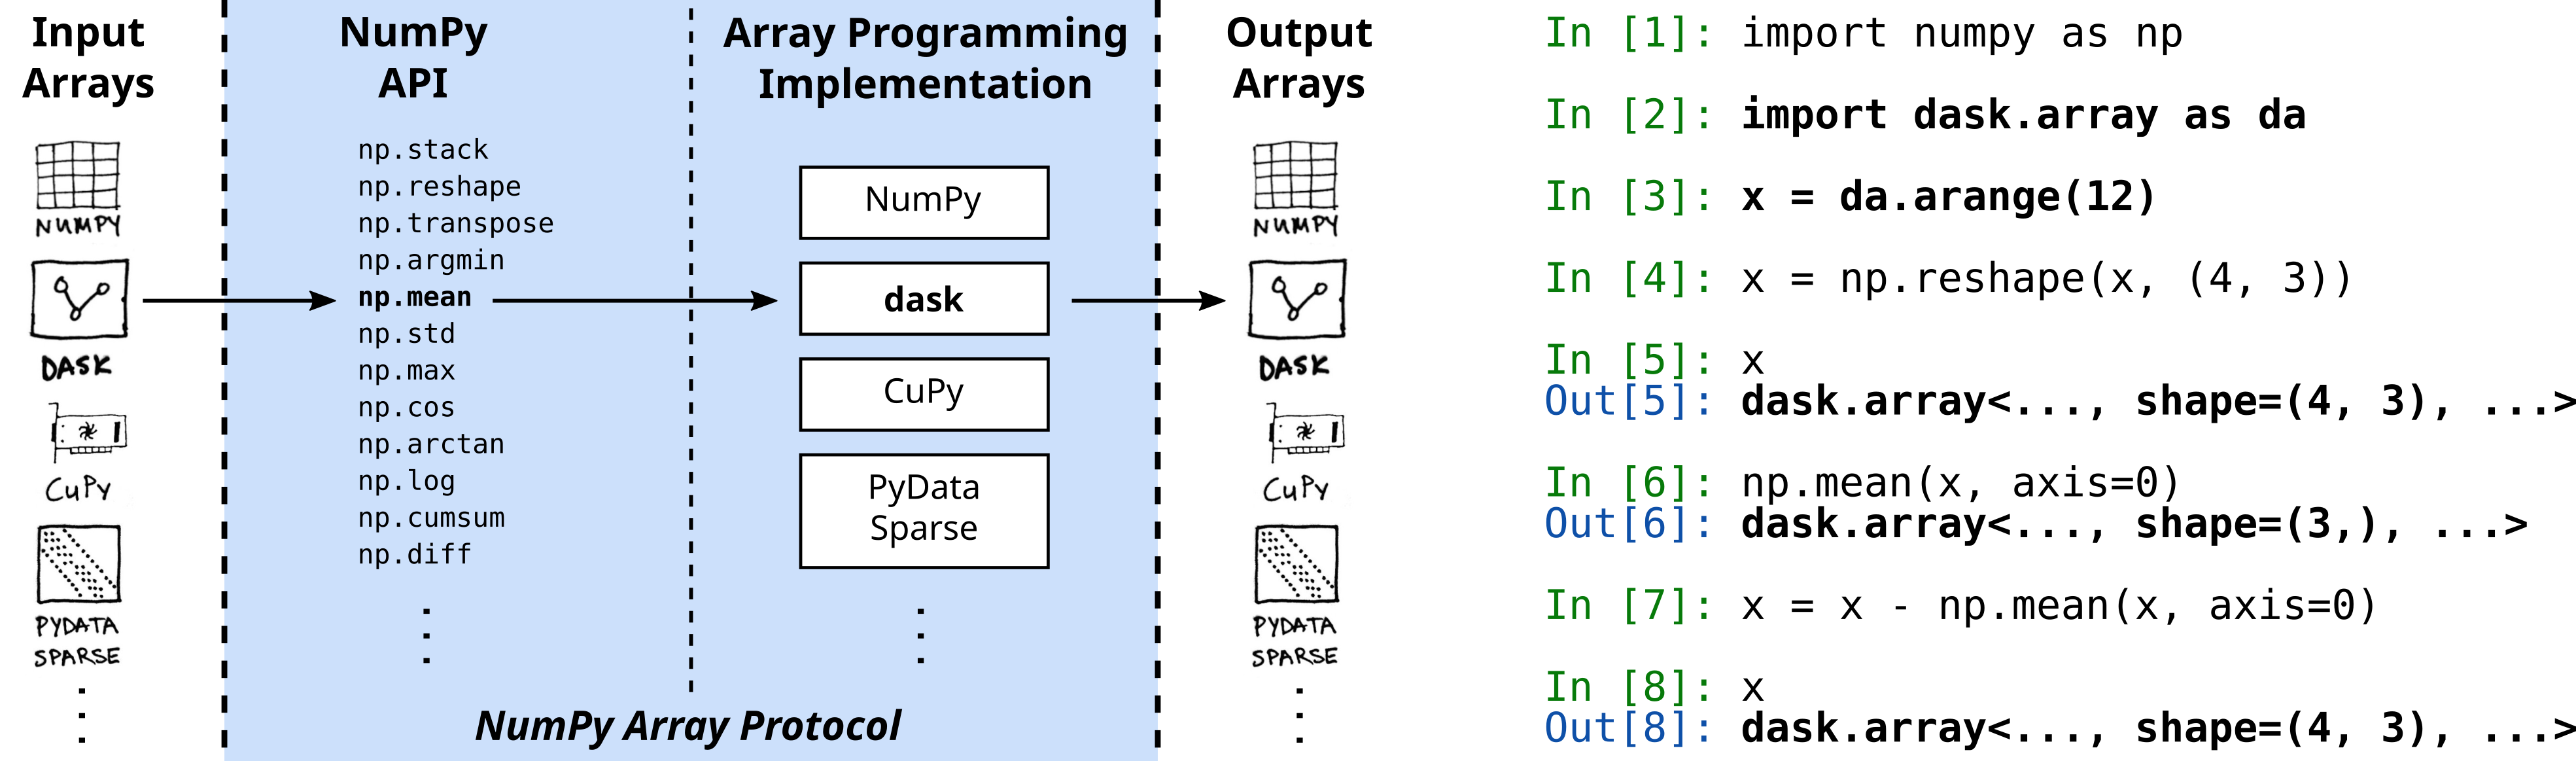
\includegraphics[width=\textwidth]{static/sketches/protocol}

  \caption{\textbf{NumPy's API and array protocols expose new arrays to the ecosystem.}
     In this example, NumPy's \texttt{mean} function is called on a Dask
     array.  The call succeeds by dispatching to the appropriate library implementation
     (i.e., Dask in this case) and results in a new Dask array.  Compare this
     code to the example code in Fig.~\ref{fig:array-concepts}g.
  }\label{fig:array-protocol}

\end{figure*}

NumPy provides in-memory, multidimensional, homogeneously typed
(i.e., single pointer and strided) arrays on CPUs.  It runs on machines
ranging from embedded devices to the world's largest supercomputers,
with performance approaching that of compiled languages.
For most its existence, NumPy addressed the vast majority of
array computation use cases.

However, scientific data sets now routinely exceed the memory capacity of a single machine and may
be stored on multiple machines or in the cloud.
In addition, the recent need to accelerate deep learning and artificial intelligence applications
has led to the emergence of specialized accelerator hardware,
including graphics processing units (GPUs), tensor processing units (TPUs),
and field-programmable gate arrays (FPGAs).
Due to its in-memory data model, NumPy is currently unable to
utilize such storage and specialized hardware directly.  However, both
distributed data and the parallel execution of GPUs, TPUs, and FPGAs map well
to the \emph{paradigm} of array programming: a gap, therefore, existed between
available modern hardware architectures and the tools necessary to
leverage their computational power.

The community's efforts to fill this gap led to a
proliferation of new array implementations. For example, each deep learning framework created
its own arrays; PyTorch \cite{NEURIPS2019_9015},
Tensorflow \cite{abadi2016tensorflow}, Apache MXNet \cite{chen2015mxnet},
and JAX arrays all have the
capability to run on CPUs and GPUs, in a distributed fashion, utilizing lazy evaluation
to allow for additional performance optimizations.  SciPy and PyData/Sparse both
provide sparse arrays---which typically contain few non-zero values and store
only those in memory for efficiency.
In addition, there are projects that build on top of NumPy arrays as a data
container and \textit{extend} its capabilities.  Distributed arrays are
made possible that way by Dask, and labeled arrays---referring to dimensions of
an array by name rather than by index for clarity, compare \texttt{x[:,~1]} vs.
\texttt{x.loc[:,~'time']}---by xarray \cite{hoyer2017xarray}.

Such libraries often mimic the NumPy API, because it lowers the
barrier to entry for newcomers and provides the wider community with a
stable array programming interface. This, in turn, prevents disruptive
schisms like the divergence of Numeric and Numarray.
But exploring new ways of working with arrays is experimental by nature
and, in fact, several promising libraries---such as Theano and Caffe---have
already ceased development. And each time that a user
decides to try a new technology, they must
change import statements and ensure that the new library implements
all the parts of the NumPy API they currently use.

Ideally, operating on specialized arrays using NumPy functions or semantics would
simply work, so that users could write code once, and would then benefit
from switching between NumPy arrays, GPU arrays, distributed arrays,
and so forth, as appropriate.
To support array operations between external array objects, NumPy
therefore added the capability to act as a central coordination
mechanism with a well-specified API (Fig.~\ref{fig:ecosystem}).

To facilitate this \emph{interoperability}, NumPy provides
``protocols'' (or contracts of operation), that allow for specialized arrays to be
passed to NumPy functions (Fig.~\ref{fig:array-protocol}).
NumPy, in turn, dispatches operations to the originating library, as required.
Over four hundred of the most popular
NumPy functions are supported.
The protocols are implemented by widely used libraries such as Dask, CuPy,
xarray, and PyData/Sparse.
Thanks to these developments, users can now, for example, scale
their computation from a single machine to distributed systems using Dask.
The protocols also \textit{compose} well, allowing users to redeploy NumPy
code at scale on distributed, multi-GPU systems via, for instance, CuPy arrays embedded in Dask
arrays. Using NumPy's high-level API, users can leverage highly parallel code
execution on multiple systems with millions of cores, all with minimal code
changes \cite{entschev2019}.

These array protocols are now a key feature of NumPy, and are expected to only
increase in importance.  As with the rest of NumPy, we iteratively refine and
add protocol designs to improve utility and simplify adoption. 

\section*{Discussion}

NumPy combines the expressive power of \emph{array programming},
the performance of C, and
the readability, usability, and versatility of Python in a mature,
well-tested, well-documented, and community-developed library.
Libraries in the scientific Python ecosystem provide fast implementations of most important algorithms.
Where extreme optimization is warranted, compiled languages such as
Cython \cite{behnel2011cython}, Numba \cite{Lam:2015:NLP:2833157.2833162},
and Pythran \cite{guelton2015pythran}, that
extend Python and transparently accelerate bottlenecks, can be
used.
Because of NumPy's simple memory model, it is easy to write low-level, hand-optimized code, usually in C
or Fortran, to manipulate NumPy arrays and pass them back to
Python.
Furthermore, using array protocols, it is possible to utilize the full
spectrum of specialized hardware acceleration with minimal changes to
existing code.

NumPy was initially developed by students, faculty, and researchers to
provide an advanced, open-source array programming library for Python,
which was free to use and unencumbered by license servers, dongles, and the like.
There was a sense of building something consequential together,
for the benefit of many others.  Participating in
such an endeavor, within a welcoming community of like-minded
individuals, held a powerful attraction for many early contributors.

These user-developers frequently had to write code from scratch to solve
their own or their colleagues' problems---often in low-level languages
that precede Python, like Fortran \cite{dongarra2008netlib} and C.
To them, the advantages of an interactive, high-level array library
were evident. The design of this new tool was informed by other
powerful interactive programming languages for scientific computing
such as Basis \cite{dubois1989basis}, Yorick \cite{munro1995using}, R \cite{ihaka1996r},
and APL \cite{iverson1962programming},
as well as commercial languages and environments like IDL and {MATLAB}.

What began as an attempt to add an array object to Python became the
foundation of a vibrant ecosystem of tools.  Now, a large amount of
scientific work depends on NumPy being correct, fast, and stable.  It
is no longer a small community project, but is core scientific
infrastructure.

The developer culture has matured: while initial development was
highly informal, NumPy now has a roadmap and a process for proposing
and discussing large changes.  The project has formal governance
structures and is fiscally sponsored by NumFOCUS, a nonprofit that
promotes open practices in research, data, and scientific computing.
Over the past few years, the project attracted its first funded
development, sponsored by the Moore and Sloan Foundations, and
received an award as part of the Chan Zuckerberg Initiative's
Essentials of Open Source Software program.  With this funding, the
project was (and is) able to have sustained focus over multiple months
to implement substantial new features and improvements.  That said, it
still depends heavily on contributions made by graduate students and
researchers in their free time.

NumPy is no longer \emph{just} the foundational array library underlying
the scientific Python ecosystem, but has also become the standard API
for tensor computation and a central coordinating mechanism between
array types and technologies in Python. Work continues to expand on and
improve these interoperability features.

Over the next decade, we will face several challenges.  New devices will be
developed, and existing specialized hardware will evolve, to meet diminishing
returns on Moore's law.  There will be more, and a wider variety of, data
science practitioners, a significant proportion of whom will be using NumPy.
The scale of scientific data gathering will continue to expand, with the
adoption of devices and instruments such as light sheet microscopes and the
Large Synoptic Survey Telescope (LSST) \cite{jenness2018lsst}.  New generation
languages, interpreters, and compilers, such as Rust
\cite{10.1145/2692956.2663188}, Julia \cite{Julia-2017}, and LLVM
\cite{LLVM:CGO04}, will invent and determine the viability of new concepts and
data structures.

Through various mechanisms described in this paper, NumPy is poised to
embrace such a changing landscape, and to continue playing a leading
role in interactive scientific computation.  To do so will require
sustained funding from government, academia, and industry.  But,
importantly, it will also need a new generation of graduate students
and other developers to engage, to build a NumPy that meets the needs
of the next decade of data science.
